\subsubsection{Missaligned Data}


\begin{center}
    \begin{figure}[h]
      \centering
      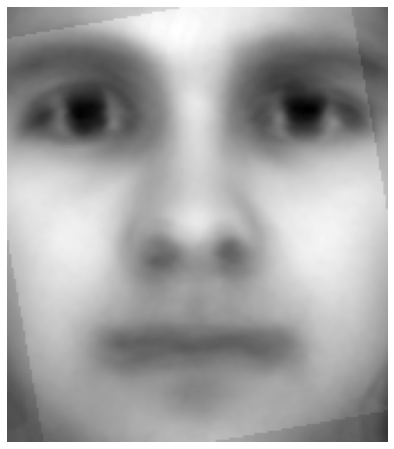
\includegraphics[width=0.94\linewidth]{external_content/media/rotation/average_face-rotation.png}
      \captionsetup{justification=centering}
      % \caption{}
      % \label{}
    \end{figure}
\end{center}


\cite{brunton2019data} (section 1.7)

\begin{itemize}
	\item Showcase Eigenfaces with rotation
	\item only few images ruin the batch
	\item the dataset was meticulously centered and optimized by hand for a proof of concept
\end{itemize}

\clearpage




\subsubsection{Too broad singular values}

\begin{center}
    \begin{figure}[h]
      \centering
      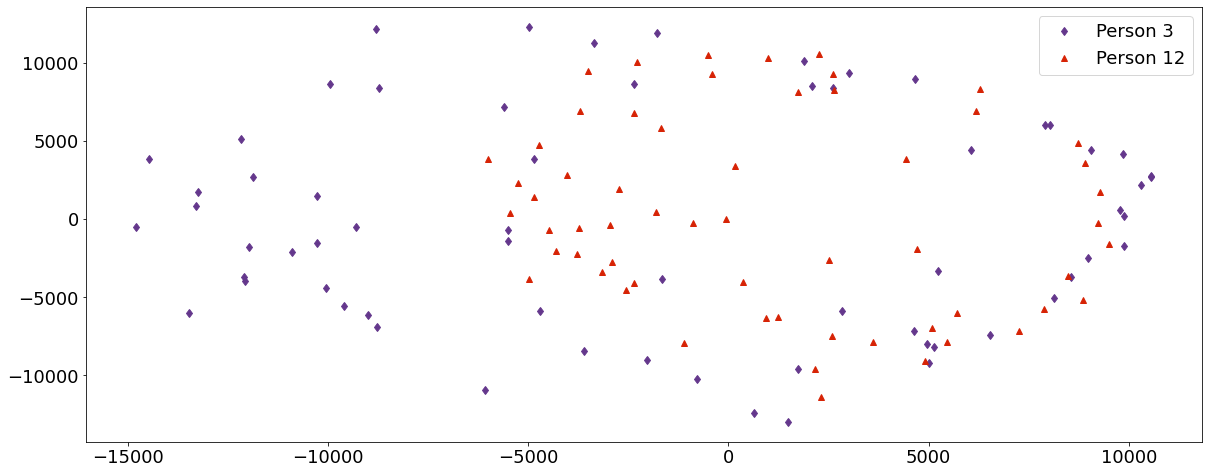
\includegraphics[width=0.94\linewidth]{external_content/media/choice_of_pc/p3_12-pc1_2-centered.png}
      \captionsetup{justification=centering}
      % \caption{}
      % \label{}
    \end{figure}
\end{center}

First principal components might be too general and not \cite{brunton2019data} (section 1.6 - last figure)

\begin{itemize}
	\item Showcase Eigenfaces distribution of the images
	\item 5 and 6 work great
	\item others ruin all the information
	\item all the vertices are one picture of a person
	\item taken with various facial expressions and very different lighting settings
\end{itemize}


\clearpage





\subsubsection{Different units}

\begin{center}
    \begin{figure}[h]
      \centering
      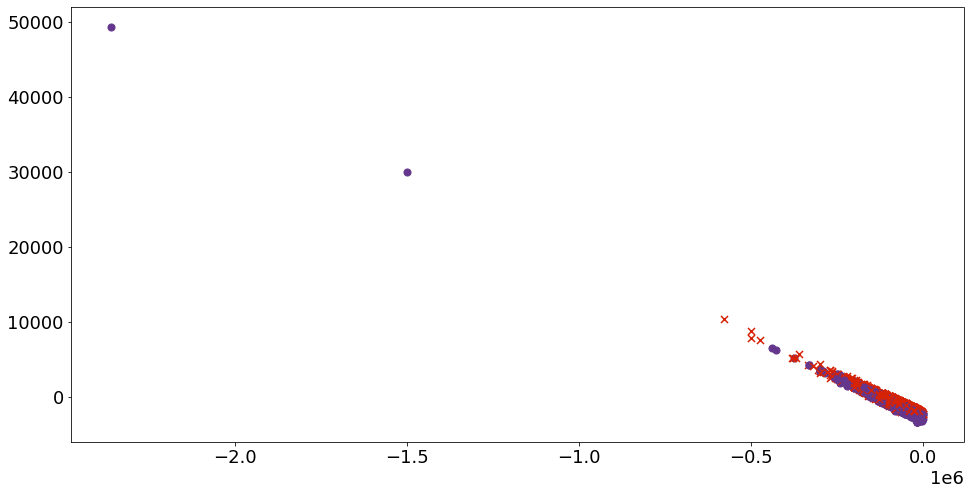
\includegraphics[width=0.94\linewidth]{external_content/media/wrong_units/graph.png}
      \captionsetup{justification=centering}
      % \caption{}
      % \label{}
    \end{figure}
\end{center}


Different units WITHIN THE MATRIX... \cite{Jolliffe2002book} (Section 2.3 page 22)

\begin{itemize}
	\item relevant for ALL the values
	\item bigger numbers become dominant no matter what
	\item example car data set. I thought I was being smart... NOPE
\end{itemize}

\clearpage
